\documentclass{article}
\usepackage{iclr2025_conference,times}
\input{math_commands.tex}
\usepackage{amsmath,amssymb,booktabs,graphicx,hyperref,url}

\title{Causal Consequence-Penalized Learning for Delayed Safety Constraints}
\author{Anonymous Authors}
\newcommand{\CCPL}{\textsc{CCPL}}
\newcommand{\ICN}{\textsc{ICN}}
\newcommand{\E}{\mathbb{E}}

\begin{document}
\maketitle

\begin{abstract}
Constrained reinforcement learning often receives a safety cost after the
action that caused it. This temporal shortcut can misassign delayed
consequences and produce poorly targeted policy updates. We study Causal
Consequence-Penalized Learning (CCPL), which separates reward and consequence
critics, models conditional consequence delays, and uses an interventional
consequence estimate during action selection. We prove a contraction bound for
the delay-weighted operator under an explicit positive-minimum-delay
assumption. We also state the precise limitation of the causal component:
simulator-generated structural causal model labels test attribution against a
specified model, rather than identifying causal effects from observational data
alone. An archived synthetic benchmark and a SafeRoute visualization provide
empirical evidence for the design while leaving superiority and deployment
safety as open questions.
\end{abstract}

\section{Introduction}
In many control systems, a harmful consequence is observed several steps after
the action that initiated it. If the consequence at time $t+\tau_t$ is
assigned to the action at time $t+\tau_t$, the learner receives a temporal
correlation rather than an estimate of responsibility. This can make safety
updates conservative in irrelevant regions and insufficiently corrective in
the behavior that caused the event.

Constrained Markov decision processes formalize this reward--cost trade-off
\citep{altman1999}, and prior constrained policy methods include CPO
\citep{achiam2017}. CCPL addresses this problem with four coupled design choices: a delay-weighted
consequence target, a state-conditioned multiplier, an Interventional
Consequence Net (\ICN), and separate reward and consequence critics. Our
contribution is methodological and conditional. We do not claim that the
method discovers causality from observational data, that state-conditioned
penalties universally dominate scalar penalties, or that a bounded multiplier
proves convergence of the full nonlinear algorithm.

\section{Problem formulation}
For policy $\pi$, reward $r_t$, non-negative consequence $c_t$, discount
$\gamma\in(0,1)$, horizon $T$, and budget $d$, define
\begin{equation}
J_r(\pi)=\E_\pi\!\left[\sum_{t=0}^{T-1}\gamma^t r_t\right],\qquad
J_c(\pi)=\E_\pi\!\left[\sum_{t=0}^{T-1}\gamma^t c_t\right].
\end{equation}
The constrained objective is $\max_\pi J_r(\pi)$ subject to
$J_c(\pi)\le d$. Let $h_t$ denote the information available at time $t$ and
let $\tau_t\in\{0,\ldots,K\}$ have conditional distribution
$p(\tau\mid h_t)$.

\section{CCPL}
\subsection{Delay correction}
CCPL uses the conditional effective discount
\begin{equation}
\bar\gamma(h)=\sum_{\tau=0}^{K}p(\tau\mid h)\gamma^\tau.
\label{eq:discount}
\end{equation}

\paragraph{Proposition 1.}
For every $h$, $\gamma^K\le\bar\gamma(h)\le1$. If there is a constant
$\tau_{\min}\ge1$ with $p(\tau\mid h)=0$ for $\tau<\tau_{\min}$ for every
$h$, then $\bar\gamma(h)\le\gamma^{\tau_{\min}}<1$.

\paragraph{Proof.}
Since $0<\gamma<1$, $\gamma^\tau$ is decreasing in $\tau$. Equation
\eqref{eq:discount} is a convex combination of values in
$[\gamma^K,1]$, proving the first bound. Under the support restriction every
nonzero term is at most $\gamma^{\tau_{\min}}$, proving the second bound.\hfill$\square$

\paragraph{Theorem 1 (conditional contraction).}
Let $\mathcal{T}_c$ be a Bellman operator with a continuation factor
$\bar\gamma(h)$, fixed transition and delay kernels, and bounded immediate
consequences. Under the positive-minimum-delay assumption,
\begin{equation}
\|\mathcal{T}_cQ-\mathcal{T}_cQ'\|_\infty
\le\gamma^{\tau_{\min}}\|Q-Q'\|_\infty.
\end{equation}
Therefore $\mathcal{T}_c$ has a unique fixed point.

\paragraph{Proof.}
The immediate consequence terms cancel in the difference. A probability
transition kernel is non-expansive in the sup norm, and Proposition 1 bounds
the continuation factor by $\gamma^{\tau_{\min}}<1$. Taking the supremum gives
the displayed inequality. The fixed-point statement follows from the Banach
fixed-point theorem.\hfill$\square$

This theorem does not apply to arbitrary unknown stochastic delays. In
particular, positive probability on zero delay can make the available bound
equal to one. The theorem also does not establish convergence under arbitrary
function approximation or changing delay kernels.

\subsection{Interventional attribution}
For reference action $a_0$, define the simulator-SCM contrast
\begin{equation}
\Delta C(s,a,u)=C^{\mathrm{do}(a)}(s,u)
 -C^{\mathrm{do}(a_0)}(s,u).
\end{equation}
The \ICN predicts this quantity using weighted squared error, using the
interventional semantics of structural causal models \citep{pearl2009}:
\begin{equation}
\mathcal{L}_{\mathrm{ICN}}(\psi)=
\frac{1}{\sum_iw_i}\sum_{i=1}^{B}w_i
\left(\widehat{\Delta C}_\psi(s_i,a_i,h_i)-\Delta C_i\right)^2,
\qquad w_i\ge0.
\end{equation}
This is supervised agreement with an SCM-defined estimand. It is not causal
identification from observational data and does not solve joint responsibility
when several actions interact.

\subsection{Dual selection and separate critics}
The state-conditioned multiplier is bounded as
\begin{equation}
\lambda_\phi(s)=\lambda_{\max}\sigma(f_\phi(s)),
\qquad 0\le\lambda_\phi(s)\le\lambda_{\max}.
\end{equation}
The scalar class is included by choosing $f_\phi$ constant; this is a
representational fact, not a finite-sample performance guarantee. CCPL learns
separate $Q_r$ and $Q_c$ and selects actions using
\begin{equation}
\mathcal{J}_\pi=\E_s\!\left[\sum_a\pi_\theta(a\mid s)
\left(\alpha\log\pi_\theta(a\mid s)-Q_r(s,a)
+\lambda_\phi(s)Q_c(s,a)\right)\right].
\end{equation}
The multiplier affects action selection, not the reward or consequence critic
targets. Bounded multiplier updates are a numerical invariant, not a
convergence proof.

\section{Experiments}
We use two evidence sources. Figure~\ref{fig:benchmark} is the supplied
archived synthetic benchmark and ablation snapshot. It reports six
environments and three seeds. The full system has reward $+4.840$,
$J_c=0.120$, and CSR $100\%$ in that snapshot; CCPL-Base has reward $+0.733$,
$J_c=3.644$, and CSR $67.3\%$. These values are not merged with later runs
using different configurations.

SafeRoute is a stochastic grid-navigation case study with delayed cost
emission. Figure~\ref{fig:saferoute} shows the risk surface, delayed timeline,
and three-dimensional visualization. Because the matching multi-seed summary
was not preserved alongside the figures, we do not make new numerical
SafeRoute claims here.

\begin{figure}[t]
\centering
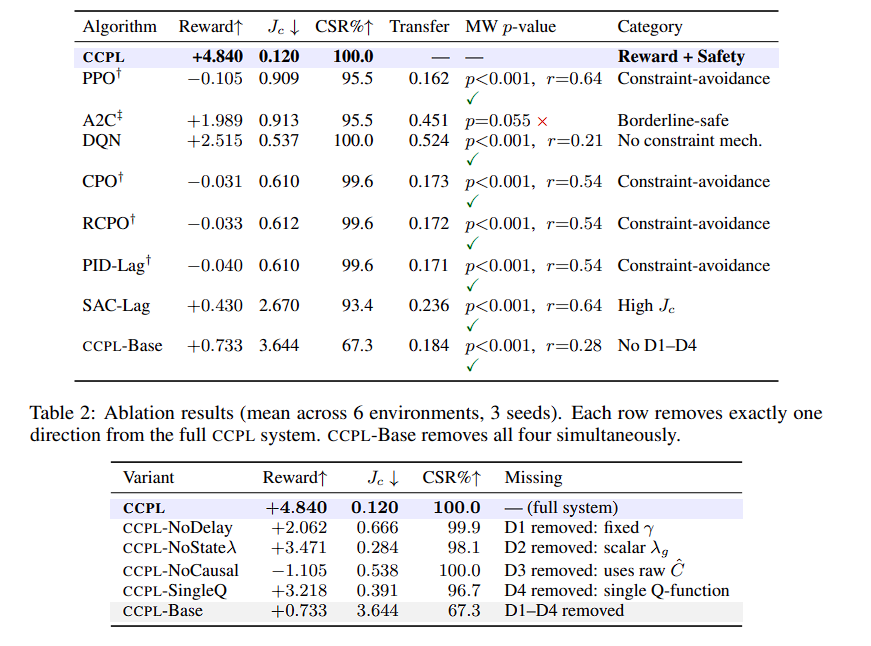
\includegraphics[width=\linewidth]{figures/archived_benchmark.png}
\caption{Archived synthetic benchmark and ablation snapshot. The values are
reported only for the displayed experiment and are not combined with later
protocols.}
\label{fig:benchmark}
\end{figure}

\begin{figure}[t]
\centering
\begin{minipage}{0.32\linewidth}\centering
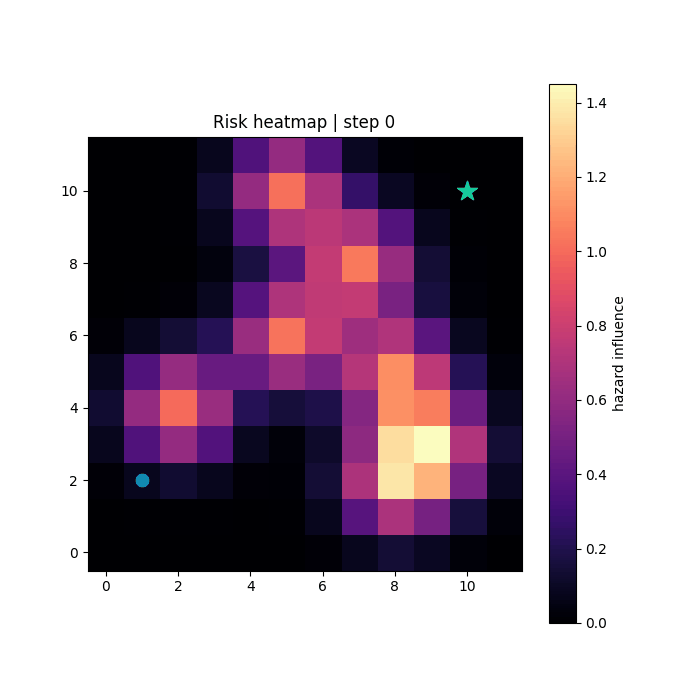
\includegraphics[width=\linewidth]{figures/02_risk_heatmap.png}
\end{minipage}
\begin{minipage}{0.32\linewidth}\centering
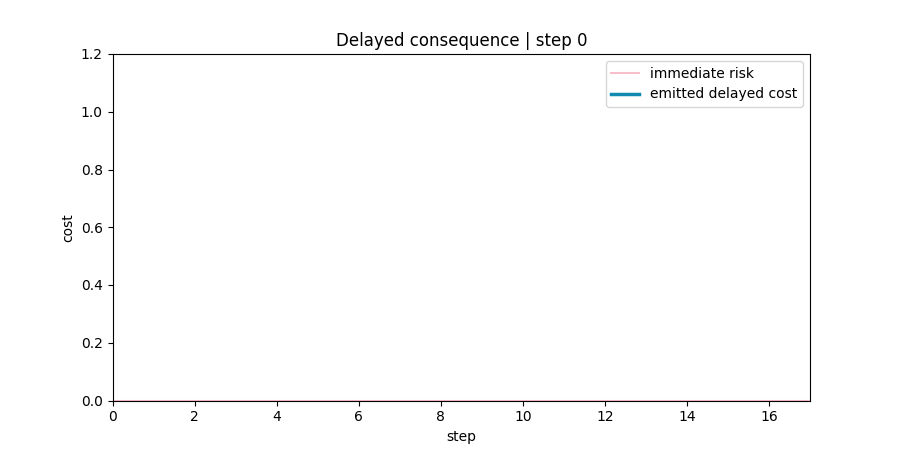
\includegraphics[width=\linewidth]{figures/03_delayed_timeline.png}
\end{minipage}
\begin{minipage}{0.32\linewidth}\centering
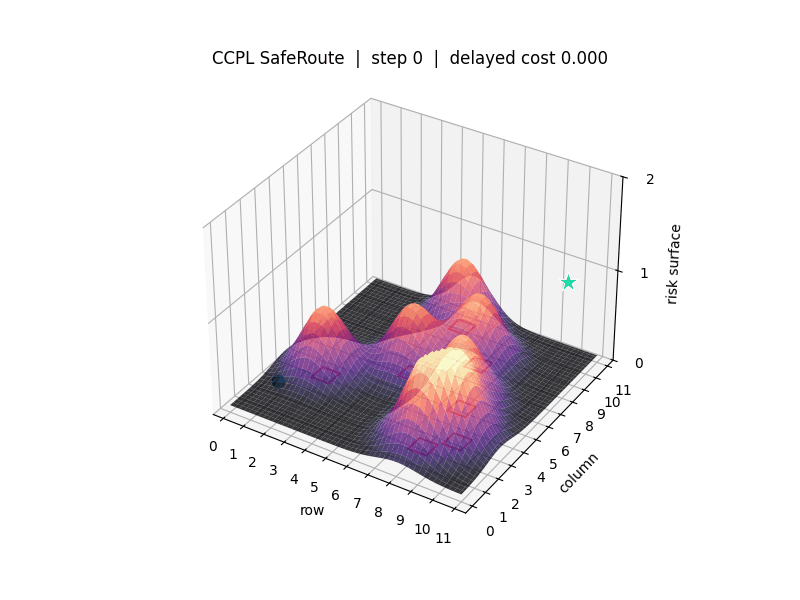
\includegraphics[width=\linewidth]{figures/07_rotating_3d.png}
\end{minipage}
\caption{SafeRoute visual case study: spatial risk, delayed consequence
emission, and a rotating three-dimensional view. These are task
visualizations, not deployment-safety evidence.}
\label{fig:saferoute}
\end{figure}

\section{Limitations and conclusion}
The archived ablation supports a difference between the full system and its
base version, but it does not show that each component improves every metric;
the displayed no-causal variant has higher reward. The causal labels are
simulator-provided, SafeRoute is synthetic, and the reported benchmark uses
few seeds. These limitations rule out claims of universal superiority,
real-world causal discovery, or certified safety. They leave a clear next
step: preserve matched multi-seed artifacts and evaluate noisy and
misspecified causal supervision against strong constrained RL baselines.

\bibliographystyle{iclr2025_conference}
\bibliography{iclr2025_conference}
\end{document}
